\documentclass[border=10pt]{standalone}

\usepackage{tikz}
\usepackage{tikzsymbols}
\usetikzlibrary{calc,patterns,shapes.geometric}

\def\centerarc[#1](#2)(#3:#4:#5){\draw[#1] ($(#2)+({#5*cos(#3)},{#5*sin(#3)})$) arc (#3:#4:#5);}

\begin{document}
	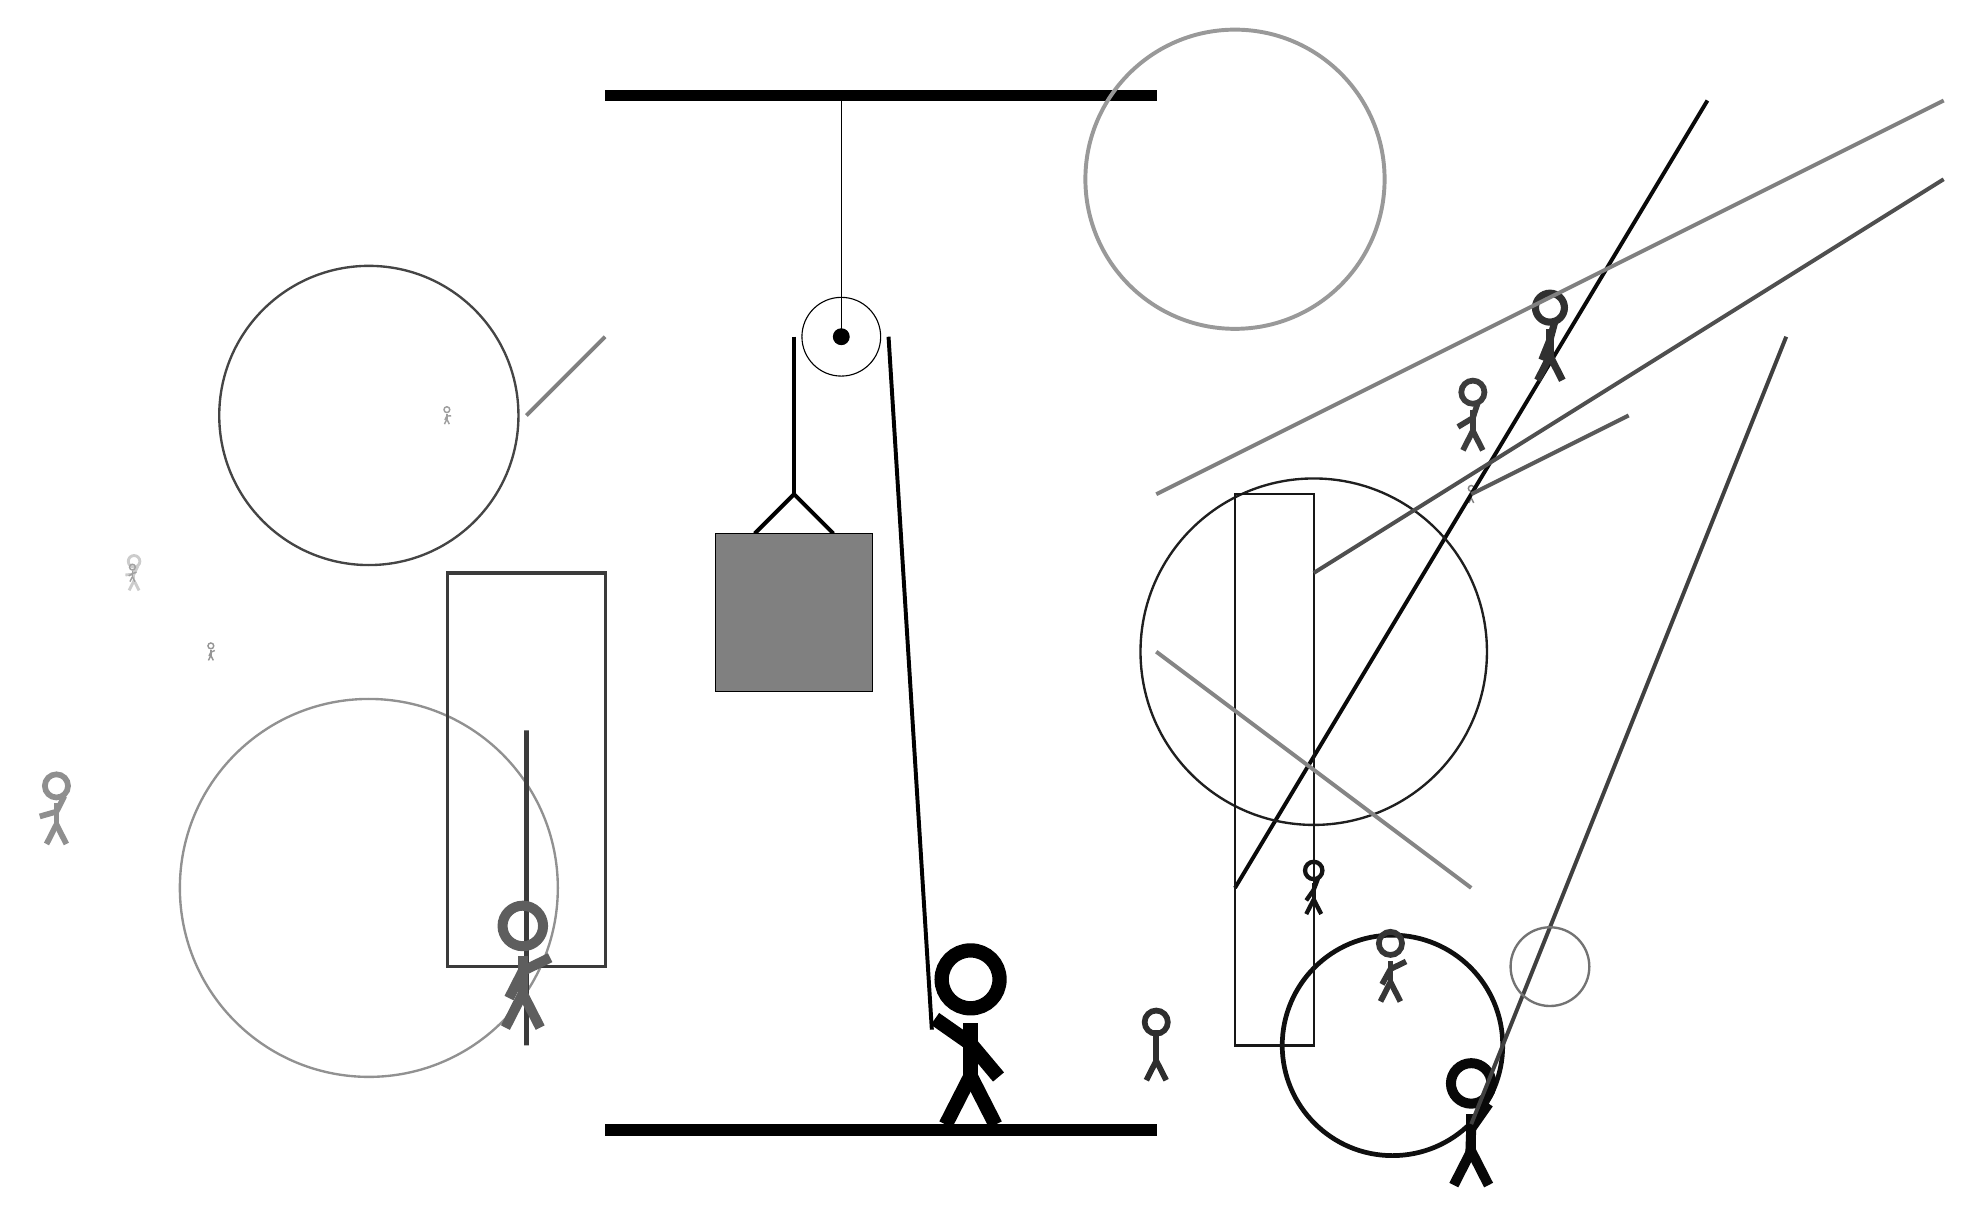
\begin{tikzpicture}
		%%%%% START %%%%%
		
		\draw[fill=black] (-2, 10) rectangle (5, 10.125);
		
		\draw (1, 7) circle (0.5);
		\draw[fill=black] (1, 7) circle (0.1);
		\draw (1, 10) -- (1, 7);
		
		\node[line width=0.6mm, color=black!49] at (9, 5) {\Strichmaxerl[1][47][50]};
		
		\draw[line width=0.5mm, color=black!96](6, 0) -- (12, 10);
		\node[line width=0.4mm, color=black!20] at (-8, 4) {\Strichmaxerl[2][5][65]};
		\node[line width=0.5mm, color=black!41] at (-7, 3) {\Strichmaxerl[1][64][25]};
		\node[line width=0.7mm, color=black!44] at (-9, 1) {\Strichmaxerl[4][16][63]};
		
		\node[line width=0.7mm, color=black!81] at (10, 7) {\Strichmaxerl[5][68][75]};
		\draw [line width=0.3mm, color=black!43](-5, 0) circle (2.4);
		\node[line width=0.7mm, color=black!76] at (9, 6) {\Strichmaxerl[4][31][72]};
		\draw[line width=0.5mm, color=black!65](9, 5) -- (11, 6);
		
		\draw[line width=0.7mm, color=black!77] (-3, -2) rectangle (-3, 2);
		\draw [line width=0.6mm, color=black!94](8, -2) circle (1.4);
		
		\draw[line width=0.5mm, color=black!50](-2, 7) -- (-3, 6);
		\node[line width=0.4mm, color=black!97] at (9, -3) {\Strichmaxerl[7][88][55]};
		
		\draw[line width=0.5mm, color=black!75](9, -3) -- (13, 7);
		\draw[line width=0.4mm, color=black!77] (-4, 4) rectangle (-2, -1);
		\draw [line width=0.3mm, color=black!88](7, 3) circle (2.2);
		
		\node[line width=0.2mm, color=black!38] at (-4, 6) {\Strichmaxerl[1][62][4]};
		
		\node[line width=0.3mm, color=black!37] at (-8, 4) {\Strichmaxerl[1][32][18]};
		\node[line width=0.2mm, color=black!63] at (-3, -1) {\Strichmaxerl[7][63][26]};
		\node[line width=0.3mm, color=black!92] at (7, 0) {\Strichmaxerl[3][55][69]};
		\draw[line width=0.3mm, color=black!91] (7, -2) rectangle (6, 5);
		
		\node[line width=0.4mm, color=black!79] at (8, -1) {\Strichmaxerl[4][61][26]};
		
		\node[line width=0.4mm, color=black!82] at (5, -2) {\Strichmaxerl[4][90][90]};
		\draw [line width=0.5mm, color=black!40](6, 9) circle (1.9);
		\draw[line width=0.5mm, color=black!69](7, 4) -- (15, 9);
		
		\draw [line width=0.3mm, color=black!73](-5, 6) circle (1.9);
		\draw[line width=0.5mm, color=black!48](9, 0) -- (5, 3);
		\draw[line width=0.5mm, color=black!50](5, 5) -- (15, 10);
		\draw [line width=0.3mm, color=black!55](10, -1) circle (0.5);
		
		\draw[line width=0.5mm] (-0.1, 4.5) -- (0.4, 5.0) -- (0.9, 4.5);
		\draw[fill=black!50] (-0.6, 4.5) rectangle (1.4, 2.5);
		
		\draw[line width=0.5mm] (0.4, 7) -- (0.4, 5.0);
		\centerarc[line width=0.5mm](1, 7)(0:180:0.6);
		\draw[line width=0.5mm](1.6, 7) -- (2.15, -1.8);
		
		\node at (2.6, -1.9) {\Strichmaxerl[10][-35][-50]};
		
		\draw[fill=black] (-2, -3) rectangle (5, -3.15);
		
		%%%%% END %%%%%
	\end{tikzpicture}
\end{document}